\documentclass[12pt]{article}
\usepackage{amsmath}
\usepackage{amsfonts}
\usepackage{amssymb}
\usepackage{subfig}
\usepackage{graphicx}
\usepackage{float}


%%%%% TIKZ CODE (For Feynman diagrams)
\usepackage{tikz}
\usetikzlibrary{arrows,shapes}
\usetikzlibrary{trees}
\usetikzlibrary{matrix,arrows} 				% For commutative diagram
											% http://www.felixl.de/commu.pdf
\usetikzlibrary{positioning}				% For "above of=" commands
\usetikzlibrary{calc,through}				% For coordinates
\usetikzlibrary{decorations.pathreplacing}  % For curly braces
\usetikzlibrary{backgrounds}  				% For showing background grid
\usepackage{pgffor}							% For repeating patterns

\usetikzlibrary{decorations.pathmorphing}	% For Feynman Diagrams
\usetikzlibrary{decorations.markings}
\usetikzlibrary{snakes}
\tikzset{
	% >=stealth', %% Different kind of arrows
    vector/.style={decorate, decoration={snake}, draw},
    fermion/.style={draw=black, postaction={decorate},
        decoration={markings,mark=at position .55 with {\arrow[draw=black]{>}}}},
    fermionbar/.style={draw=black, postaction={decorate},
        decoration={markings,mark=at position .55 with {\arrow[draw=black]{<}}}},
    fermionnoarrow/.style={draw=black},
    gluon/.style={decorate, draw=
        decoration={coil,amplitude=4pt, segment length=5pt}},
    scalar/.style={dashed,draw=black, postaction={decorate},
        decoration={markings,mark=at position .55 with {\arrow[draw=black]{>}}}},
    scalarbar/.style={dashed,draw=black, postaction={decorate},
        decoration={markings,mark=at position .55 with {\arrow[draw=black]{<}}}},
    scalarnoarrow/.style={dashed,draw=black},
%
%% 	Special vectors (when you need to fine-tune wiggles)
	provector/.style={decorate, decoration={snake,amplitude=2.5pt}, draw},
	antivector/.style={decorate, decoration={snake,amplitude=-2.5pt}, draw},
}



\textwidth 6.5in
\oddsidemargin 0in
\evensidemargin 0in
\textheight 8.6in
\topmargin -0.5in
\pagestyle{empty}
\begin{document}

\vspace*{-1cm}
\begin{center}
{\LARGE \bf Relativistic Quantum Field Theory}

\vspace*{0.5cm}
{\Large Physics 7651} \\
\vspace*{0.5cm}
{\Large {\bf Homework 6}\\
\vspace*{0.5cm}
Due: In class on Wednesday, October 12}
\end{center}
\begin{enumerate}


\item  {\bf Feynman rules for a theory with complex scalars} [5 points]

In class we derived the Feynman rules for a real scalar field. We will now derive the rules for a theory with both complex fields $\psi$ and real fields $\phi$ and Lagrangian
$$
\mathcal L = \frac 12 \left(\partial \phi\right)^2  + \frac 12 m^2\phi^2 + \left|\partial \psi\right|^2 - M^2 |\psi|^2 - g\phi\psi^\dagger\psi
$$
Draw real scalar propagators as dashed lines and complex scalar propagators as solid lines with arrows pointing along the direction of U(1) charge flow:

\begin{center}
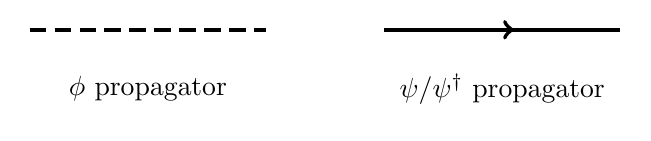
\begin{tikzpicture}[scale=1.5, line width=1.5pt]
	\draw[dash pattern = on 6 pt off 3 pt] (0,0) -- (2,0);
	\draw[fermion] (3,0) -- (5,0);
	\node at (1,-.5) {$\phi$ propagator};
	\node at (4,-.5) {$\psi$/$\psi^\dag$ propagator};
\end{tikzpicture}
\end{center}

\begin{enumerate}
\item Determine all the Feynman rules for this theory.
\item Draw and calculate the leading order diagram(s) in $g$ for $\psi\psi^\dag \to \phi\phi$. Can you draw a diagram for $\psi\psi\to \phi\phi$?
\item Draw and calculate the leading order diagram(s) in $g$ for $\psi\phi \to \psi\phi$. Can you draw a diagram for $\psi\phi \to \psi^\dag\phi$?
\item Suppose I told you that I can draw a diagram for $$p \psi\, \bar p \psi^\dag \, r \phi \to q \psi \, \bar q \psi^\dag \, s \phi,$$ where the coefficients are just the number of initial and final state particles. What relation must hold between the coefficients? Motivate this by appealing to a symmetry principle.

\end{enumerate}

\item {\bf A toy model of meson interactions} [5 points]

The most common decay mode of the $K_S$ neutral kaon ($m_{K_S} = 498$ MeV) is into two charged pions ($m_{\pi^\pm} = 145$ MeV) with a rate of $\Gamma = 0.776 \times 10^{10} \text{ sec}^{-1}$. Model this system in terms of the theory in Problem 1 with $\phi$ representing $K_S$, $\psi$ representing $\pi^+$ and $\psi^\dag$ representing $\pi^-$. Compute the dimensionless quantity $g/m_{K_S}$ and comment on why we call this is a ``weak interaction.'' \textit{Hint:} $\hbar = 6.58 \times 10^{-22}$ MeV sec.

\vspace{.5cm}

%\item {\bf Some cross section calculations} [10 points]
%
%We can now continue to connect the theory in Problem 1 to experimental observables. 
%
%\begin{enumerate}
%\item Compute, to leading order in $g$, the center-of-mass differential cross section and total cross section for the elastic scattering of $\psi\psi^\dag$.
%\item Do the same for $\psi\psi^\dag$ annihilating into $\phi\phi$. \textit{Hint:} you already calculated the amplitude in Problem 1b. Be careful not to double-count final states.
%\end{enumerate}
%
%\item {\bf Kinematics of a simple theory} [10 points]
%
%Let $A$, $B$, $C$, and $D$ be four real scalar fields with dynamics determined by the Lagrangian
%$$\mathcal L = \frac 12 \left[
%(\partial A)^2 - m^2 A^2
%+ (\partial B)^2
%+ (\partial C)^2
%+ (\partial D)^2
%\right]
%+ g ABCD,
%$$
%where $m$ and $g$ are positive real numbers. Note that $A$ is massive while $B$, $C,$ and $D$ are massless so that the decay $A\to BCD$ is allowed. Compute, to the lowest non-vanishing order in $g$, the total decay width of the $A$. How would the answer have differed if the interaction were instead $gAB^3$?

\item {\bf Models of $2\to 4$ at a real scalar collider} [10 points]

Consider the usual $\phi^4$ theory of a real scalar field,
$$
\mathcal L = \frac 12 \left(\partial \phi\right)^2  + \frac 12 m^2\phi^2 + \frac{\lambda}{4!} \phi^4.
$$
Suppose we have a $\phi$ collider and we'd like to study this theory by colliding pairs of $\phi$.
\begin{enumerate}
\item Draw the leading order diagrams for $2\to 4$ scattering. Label the external states with distinct momenta.
\item Calculate the amplitude for this process.
\item Now consider a slightly different theory with two real fields, $\phi$ and $\varphi$,
$$
\mathcal L = \frac 12 \left(\partial \phi\right)^2  + \frac 12 m^2\phi^2
+ \frac 12 \left(\partial \varphi\right)^2  + \frac 12 M^2\varphi^2
 + \frac{\lambda}{3!} \phi^3\varphi.
$$
Determine the amplitude for $2\phi \to 4\phi$ in this modified theory.
\item Suppose the mass of the $\varphi$ is much heavier than the energies of our $\phi$ collider. That is, consider the limit where $M$ is much larger than the external momenta. Write the $2\phi \to 4\phi$ amplitude in this limit. 
\item When the $\varphi$ field is too heavy to produce directly, physicists must make sense of their data by writing `effective theories' of only the low energy ($\phi$) fields. Suppose physicists at our real scalar collider observe $2\phi \to 4\phi$ scattering \textit{without} observing $2\phi \to 2\phi$ scattering. This disfavors the $\phi^4$ model so that one might consider a different effective model of $\phi$ fields such as,
$$
\mathcal L = \frac 12 \left(\partial \phi\right)^2  + \frac 12 m^2\phi^2 +\frac{g}{6!}\phi^6.
$$
What is the dimension of the coupling $g$? Suppose the actual theory of nature is that in part (d). What is the relation between the `effective coupling' parameter $g$ and the parameters of the actual theory?
\end{enumerate}


\item {\bf A theory with a derivative interaction} [10 points]

Work out the Feynman rules for the following theory of a real scalar field $\phi$,
$$
\mathcal L =
\frac 12 \left(\partial \phi\right)^2   
  + \frac{\lambda}{4}(\phi\partial\phi)^2.
$$
What is the dimension of the coupling $\lambda$? What is the amplitude for elastic $2\to 2$ scattering to first order in $\lambda$?

\textit{Hint, Oct 9.} Even though the action is Lorentz invariant, there are subtleties regarding Lorentz covariance of the interaction Hamiltonian. (See Preskill 4.33 for a discussion.) For the purposes of this problem, assume that $H_\text{int}=-\mathcal L_\text{int}$. Ignore terms coming from $\partial_0$ acting on time ordering symbols (alternately, assume the four-point term contracts with external states). Thanks to Michael for pointing this out.

\end{enumerate}

\end{document}
